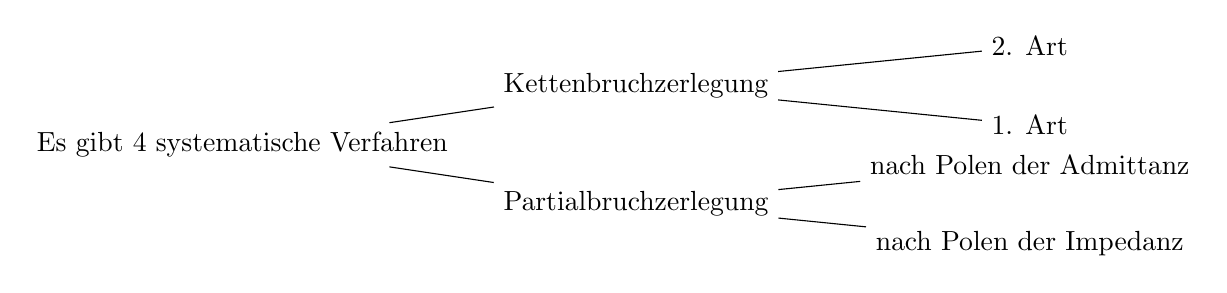
\begin{tikzpicture}[level distance=50mm,
level 1/.style={sibling distance=15mm},
level 2/.style={sibling distance=10mm}]
	\node {Es gibt 4 systematische Verfahren}[grow=right]
		child {node {Partialbruchzerlegung}
			child {node {nach Polen der Impedanz}}
			child {node {nach Polen der Admittanz}}
		}
		child {node {Kettenbruchzerlegung}
			child {node {1. Art}}
			child {node {2. Art}}
		};
\end{tikzpicture}\\